\documentclass[compress]{beamer}%compress表示尽量压缩导航条
%\usetheme{Berlin}
\usepackage{thubeamer}
\usepackage{pgf}
\usepackage[UTF8,noindent]{ctex}%取消首行缩进
\usepackage{dot2texi}
\usepackage{tikz}
\usetikzlibrary{shapes,arrows}
\usepackage{listings}
\usepackage{xcolor}
\usepackage{multicol}
\lstset{
    language=[LaTeX]TeX, 
    tabsize=4, 
    frame=shadowbox, %把代码用带有阴影的框圈起来 
    commentstyle=\color{red!50!green!50!blue!50}, %浅灰色的注释 
    rulesepcolor=\color{red!20!green!20!blue!20},%代码块边框为淡青色 
    keywordstyle=\color{blue!90}\bfseries, %代码关键字的颜色为蓝色,粗体 
    showstringspaces=false,%不显示代码字符串中间的空格标记 
    stringstyle=\ttfamily, % 代码字符串的特殊格式 
    keepspaces=true, % 
    breakindent=22pt, % 
    numbers=left,%左侧显示行号 往左靠,还可以为right,或none,即不加行号 
    stepnumber=1,%若设置为2,则显示行号为1,3,5,即stepnumber为公差,默认stepnumber=1 
    %numberstyle=\tiny, %行号字体用小号 
    numberstyle={\color[RGB]{0,192,192}\tiny} ,%设置行号的大小,大小有tiny,scriptsize,footnotesize,small,normalsize,large等
    numbersep=8pt, %设置行号与代码的距离,默认是5pt 
    basicstyle=\tiny,%\footnotesize, % 这句设置代码的大小 
    showspaces=false, % 
    flexiblecolumns=true, % 
    breaklines=true, %对过长的代码自动换行 
    breakautoindent=true,% 
    breakindent=4em, % 
    aboveskip=1em, %代码块边框 
    backgroundcolor=\color[RGB]{245,245,244}, %代码背景色 
    %backgroundcolor=\color[rgb]{0.91,0.91,0.91} %添加背景色 
}

\usepackage{times} %设置文档中的所有英文为Times new roman字体
\usefonttheme{professionalfonts}    % 设置公式中的数学字体(wenzhong) http://bbs.ctex.org/forum.php?mod=viewthread&tid=76917

\setCJKsansfont[ItalicFont={KaiTi}]{SimSun}
%\logo{
\includegraphics[width=1.3cm,height=1.3cm]{logo.pdf}} %在每个页面的右下角插入logo
\usepackage{caption}
\setbeamertemplate{caption}[numbered]{}% Number float-like environments

\begin{document}

\graphicspath{{figures/}} % figures path
\captionsetup[figure]{font=footnotesize,labelfont=footnotesize}

\title{{\LaTeX}科技论文写作简介}
\author[张三]{汇报人:张三\\ \vskip 5pt 导\quad 师:李四}
\institute[国防科技大学]{\small \vskip 38pt 国防科技大学}
\date{\small \vskip -22pt \today}
%\titlegraphic{
\includegraphics{logo.pdf}}
%\frame{
\begin{frame}
	\vspace{-10mm}
		\maketitle
	\vspace{-44mm}
	\begin{figure}[htbp]
		\begin{center}
			
\includegraphics[width=0.14\linewidth]{logo.png}
		\end{center}
	\end{figure}
\end{frame}
\section*{目录}
\begin{frame}
	\frametitle{\secname}
    \tableofcontents[]%sections={<1-5>}]
\end{frame}
 
\AtBeginSection[] {%在每一节前面加入目录显示当前节的目录结构
	\begin{frame}
		\frametitle{目录}
		\tableofcontents[currentsection,currentsubsection,hideothersubsections,sectionstyle=show/shaded,]
		\addtocounter{framenumber}{-1}  %目录页不计入页码
	\end{frame}
}

\section{什么是\LaTeX}

\begin{frame}{\secname}
    \begin{block}{\LaTeX 文档排版系统}
        \begin{itemize}
            \item LaTeX(音译“雷太赫”)是一种高质量的文档排版系统 \\
            \item 主要用于科技文档的出版和交流,目前已成为\textcolor{red}{事实上的标准}
        \end{itemize}
    \end{block}
    \begin{block}{小论文投稿时}
        \begin{itemize}
            \item 大部分期刊接收Word或LaTeX格式的稿件 \\
            \item 部分英文期刊只接收LaTeX格式的稿件
        \end{itemize}
    \end{block}
\end{frame}

\begin{frame}[fragile]{\LaTeX 工作流程}
    \begin{itemize}
        \item 将论文内容写成源文件
        \item 调用编译器,生成pdf文档
    \end{itemize}
    \begin{figure}[htbp]
        \centering
        \begin{dot2tex}[dot]
            digraph {
                rankdir = LR;
                src [shape = box, label = "源文件"];
                compile [shape = box, label = "编译"];
                pdf [shape = box, label = "pdf 文档"];
            
                src -> compile -> pdf;
            }
        \end{dot2tex}
    \end{figure}
\end{frame}

\begin{frame}[fragile]{一个简单的例子}
    \begin{columns}
        \begin{column}{0.5\textwidth}
            \begin{lstlisting}
\documentclass{article} % 文档模板
\usepackage{graphicx} % 引用宏包
\usepackage{amsmath}
% 文档标题
\title{An Simple {\LaTeX} Example} 
\author{Sun}    % 作者

\begin{document}
\maketitle  % 生成标题

\section{Introduction} % 节标题
Hello world!
\section{Equation}
\begin{equation}    % 插入公式
    a = b + c
\end{equation}
\section{Figure}
\begin{figure}[htbp] % 插入图片
    \centering
    
\includegraphics[width=0.5\textwidth]{logo.png}
    \caption{NUDT} % 图标题
\end{figure}
\end{document}
            \end{lstlisting}
        \end{column}
        \begin{column}{0.5\textwidth}
            \fbox{%
                \parbox{0.9\textwidth}{%
            \begin{figure}
                \centering
                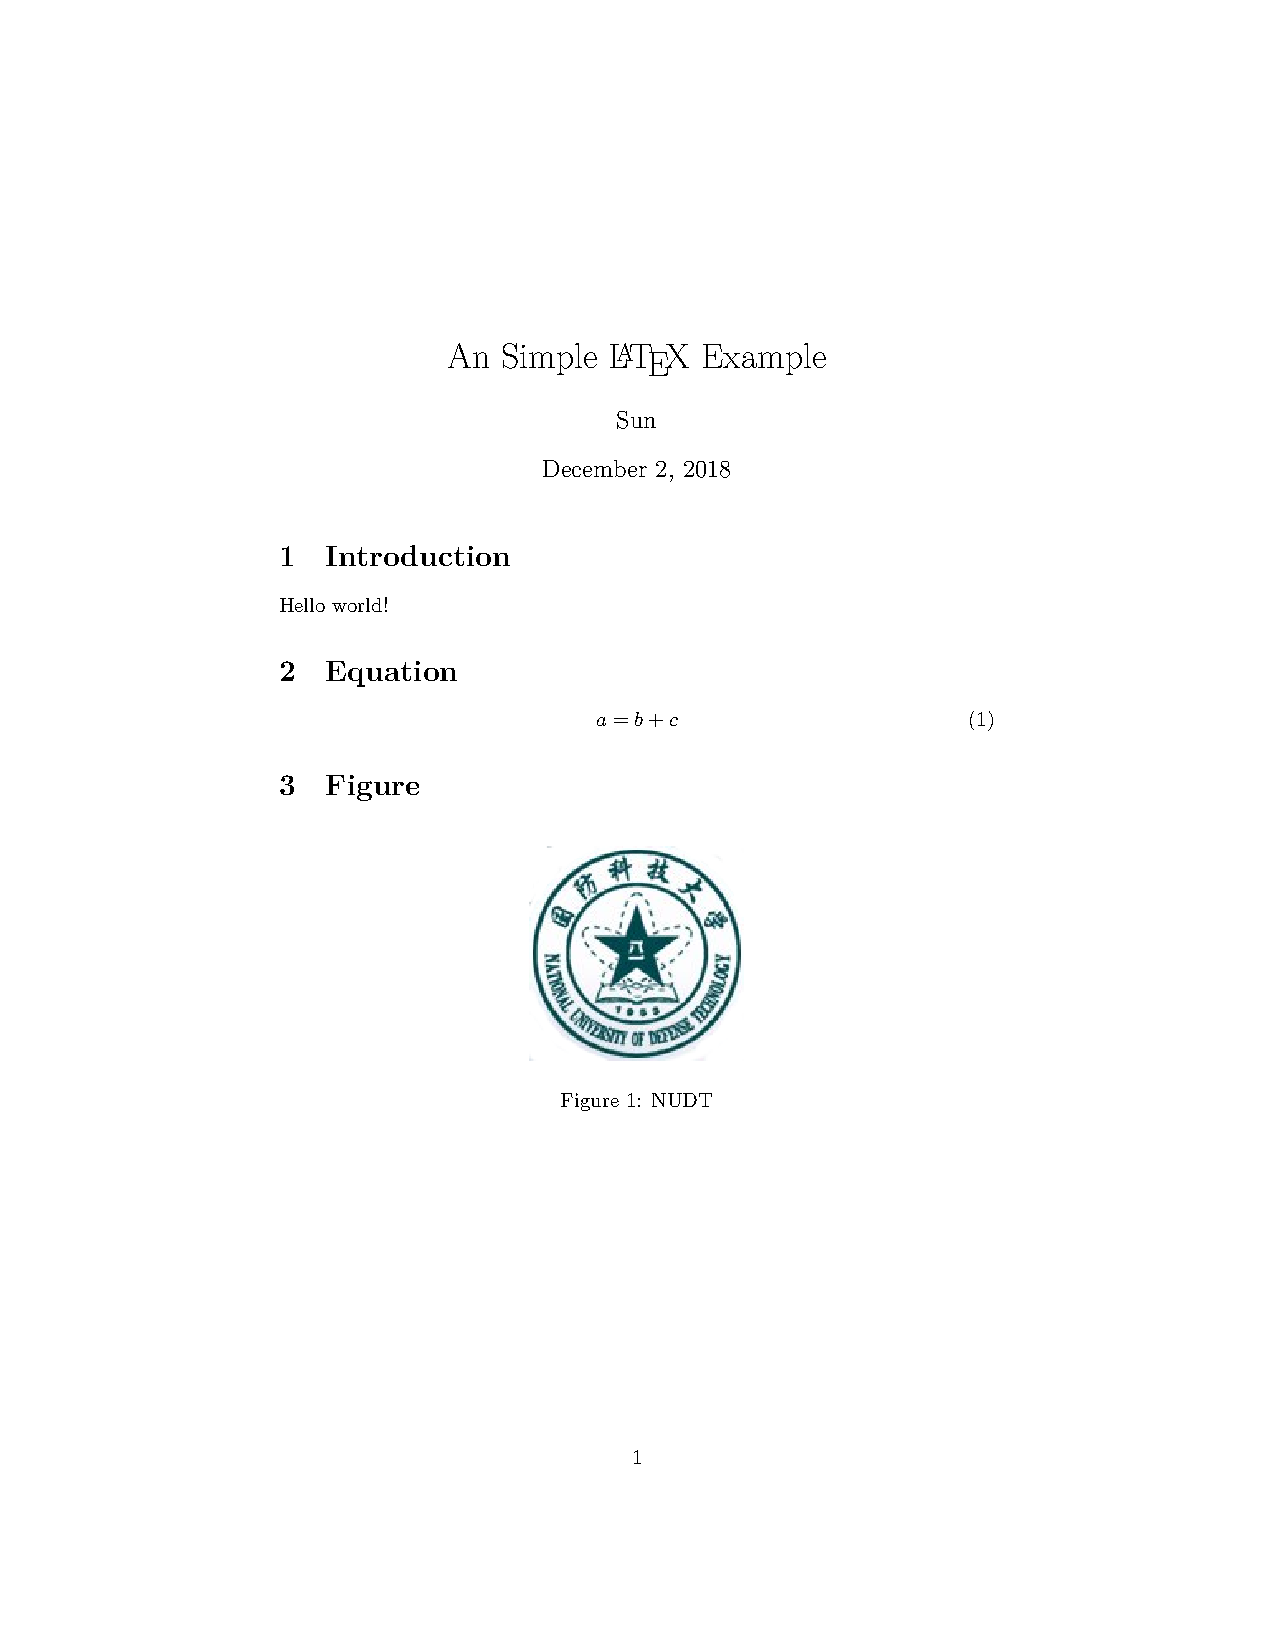
\includegraphics[width=0.8\textwidth]{example_1.pdf}
            \end{figure}
                }
            }
        \end{column}
    \end{columns}
\end{frame}

\begin{frame}{疑问}
    \begin{block}{使用Word处理文档}
        \begin{itemize}
            \item 所见即所得,不需要编译,更加直观、方便
            \item 容易上手,有很好的使用基础
            \item 功能强大,同样能达到很好的效果
        \end{itemize}
    \end{block}
    \textcolor{red}{\emph{\LARGE{为什么要用\LaTeX ?}}}
\end{frame}

\section{为什么要用\LaTeX}

\begin{frame}[fragile]{文档注释}
    \begin{columns}
        \begin{column}{0.5\textwidth}
            \begin{block}{Word}
                \begin{itemize}
                    \item 正文中不能添加注释
                    \item 审阅模式添加批注
                \end{itemize}
            \end{block}
            \begin{block}{\LaTeX}
                \begin{itemize}
                    \item 直接在源文件中添加注释,以\% 开头
                    \item 便于组织论文,整理思路
                \end{itemize}
            \end{block}
        \end{column}
        \begin{column}{0.5\textwidth}
            \begin{lstlisting}
\documentclass{article} % 文档模板
\usepackage{graphicx} % 引用宏包
\usepackage{amsmath}
% 文档标题
\title{An Simple {\LaTeX} Example} 
\author{Sun}    % 作者

\begin{document}
\maketitle  % 生成标题

\section{Introduction} % 节标题
Hello world!
\section{Equation}
\begin{equation}    % 插入公式
    a = b + c
\end{equation}
\section{Figure}
\begin{figure}[htbp] % 插入图片
    \centering
    
\includegraphics[width=0.5\textwidth]{logo.png}
    \caption{NUDT} % 图标题
\end{figure}
\end{document}
            \end{lstlisting}
        \end{column}
    \end{columns}
\end{frame}

\begin{frame}[fragile]{数学公式}
    \begin{columns}
        \begin{column}{0.5\textwidth}
            \begin{block}{Word}
                \begin{itemize}
                    \item 借助MathType实现
                    \item 多个文档之间拷贝,容易出现格式、交叉引用等问题
                \end{itemize}
            \end{block}
            \begin{block}{\LaTeX}
                \begin{itemize}
                    \item 直接在源文件中输入公式
                    \item 为每个公式定义\textcolor{red}{标签},通过标签实现交叉引用
                    \item 模板\textcolor{red}{自动编号和排序}
                \end{itemize}
            \end{block}
        \end{column}
        \begin{column}{0.5\textwidth}
            \begin{lstlisting}
\begin{equation}    % 加法公式
    \label{eq:add}
    a + b = c
\end{equation}

\begin{equation}    % 减法公式
    \label{eq:minus}
    a - b = c
\end{equation}

\begin{equation}    % 乘法公式
    \label{eq:times}
    a \times b = c
\end{equation}

式\eqref{eq:add}是一个加法公式,
式\eqref{eq:add}是一个减法公式,
式\eqref{eq:times}是一个乘法公式,
除法公式形如$a \div b = c$。
            \end{lstlisting}
        \end{column}
    \end{columns}
\end{frame}

\begin{frame}[fragile]{数学公式}
    \begin{columns}
        \begin{column}{0.5\textwidth}
            \begin{lstlisting}
\begin{equation}    % 加法公式
    \label{eq:add}
    a + b = c
\end{equation}

\begin{equation}    % 减法公式
    \label{eq:minus}
    a - b = c
\end{equation}

\begin{equation}    % 乘法公式
    \label{eq:times}
    a \times b = c
\end{equation}

式\eqref{eq:add}是一个加法公式,
式\eqref{eq:minus}是一个减法公式,
式\eqref{eq:times}是一个乘法公式,
除法公式形如$a \div b = c$。
            \end{lstlisting}
        \end{column}
        \begin{column}{0.5\textwidth}
            \fbox{%
                \parbox{\textwidth}{%
                    \begin{equation}    % 加法公式
                        \label{eq:add}
                        a + b = c
                    \end{equation}

                    \begin{equation}    % 减法公式
                        \label{eq:minus}
                        a - b = c
                    \end{equation}

                    \begin{equation}    % 乘法公式
                        \label{eq:times}
                        a \times b = c
                    \end{equation}

                    式\eqref{eq:add}是一个加法公式,
                    式\eqref{eq:minus}是一个减法公式,
                    式\eqref{eq:times}是一个乘法公式,
                    除法公式形如$a \div b = c$。
                }
            }
        \end{column}
    \end{columns}
\end{frame}

\begin{frame}[fragile]{图表排版和引用}
    \begin{columns}
        \begin{column}{0.5\textwidth}
            \begin{block}{Word}
                \begin{itemize}
                    \item 插入题注,实现图表编号、交叉引用
                    \item 多个文档之间拷贝,容易出现格式、交叉引用等问题
                    \item 图文混排,要\textcolor{red}{自己调整版式},尽量减少空白
                    \item 前文变化后,\textcolor{red}{后文要仔细检查},甚至重新排版
                \end{itemize}
            \end{block}
        \end{column}
        \begin{column}{0.5\textwidth}
            \begin{block}{\LaTeX}
                \begin{itemize}
                    \item 为每个图表定义标签,通过标签实现交叉引用
                    \item 模板会\textcolor{red}{自动调整图文混排的版式},减少空白
                    \item 前文变化后,编译时自动重新排版
                    \item 作者只需\textcolor{red}{专注于论文内容},版式由模板自动调整
                \end{itemize}
            \end{block}
        \end{column}
    \end{columns}
\end{frame}

\begin{frame}[fragile]{图表排版和引用}
    \begin{columns}
        \begin{column}{0.5\textwidth}
            \begin{lstlisting}
\begin{figure}[htb]
    \centering
    
\includegraphics[width=0.8\textwidth]{logo.png}
    \caption{国防科技大学校徽1} % 图标题
    \label{fig:NUDT_logo}
\end{figure}

\begin{figure}[htb]
    \centering
    
\includegraphics[width=0.8\textwidth]{logo1.png}
    \caption{国防科技大学校徽2} % 图标题
    \label{fig:NUDT_logo1}
\end{figure}

图\ref{fig:NUDT_logo}和图\ref{fig:NUDT_logo1}是国防科技大学校徽。
            \end{lstlisting}
        \end{column}
        \begin{column}{0.5\textwidth}
            \fbox{%
                \parbox{\textwidth}{%
                    \begin{figure}[htb]
                        \centering
                        
\includegraphics[width=0.2\textwidth]{logo.png}
                        \caption{国防科技大学校徽1} % 图标题
                        \label{fig:NUDT_logo}
                    \end{figure}

                    \begin{figure}[htb]
                        \centering
                        
\includegraphics[width=0.2\textwidth]{logo1.png}
                        \caption{国防科技大学校徽2} % 图标题
                        \label{fig:NUDT_logo1}
                    \end{figure}

                    图\ref{fig:NUDT_logo}和图\ref{fig:NUDT_logo1}是国防科技大学校徽。
                }
            }
        \end{column}
    \end{columns}
\end{frame}

\begin{frame}[fragile]{参考文献}
    \begin{columns}
        \begin{column}{0.5\textwidth}
            \begin{block}{Word}
                \begin{itemize}
                    \item \textcolor{red}{手动排列},列表变化时需要修改每一处相关引用
                    \item \textcolor{red}{编号列表}方式,可以自动编号、交叉引用
                    \item 正文调整后,\textcolor{red}{文献列表的顺序}需要手动调整
                    \item \textcolor{red}{参考文献格式},根据期刊模板,仔细调整每一条参考文献的格式
                \end{itemize}
            \end{block}
        \end{column}
        \begin{column}{0.5\textwidth}
            \begin{block}{\LaTeX}
                \begin{itemize}
                    \item 数据库 -- 标签 -- 索引
                    \item 将条目信息写入数据库文件
                    \item 正文从数据库中索引条目标签,自动生成列表和引用
                    \item 模板自动确定\textcolor{red}{引用格式},姓名+年份 / 列表序号
                    \item 列表自动生成,根据正文内容\textcolor{red}{自动调整顺序}
                    \item 根据模板格式\textcolor{red}{自动生成文献条目},不需要手动调整格式
                \end{itemize}
            \end{block}
        \end{column}
    \end{columns}
\end{frame}

\begin{frame}[fragile]{参考文献}
    \begin{multicols}{2}
    文献数据库文件 *.bib
        \begin{lstlisting}
@book{companion,
  title = {The \LaTeX Companion},
  publisher = {Addison-Wesley ...},
  year = {1994},
  author = {Michel Goosens and ...},
  pages = {112-125},
  address = {Reading, MA}
}

@inbook{berz_modern_1999,
  address = {London},
  title = {Modern Map Methods ...},
  publisher = {Academic Press},
  author = {Martin Berz},
  year = {1999},
  pages = {81-118}
}

@article{wittig_high_2015,
  title = {High order transfer ...},
  volume = {122},
  number = {4},
  journal = {Celestial Mechanics ...},
  author = {Wittig, Alexander and ...},
  year = {2015},
  pages = {333--358},
}

@phdthesis{johannes_grote,
  title = {High-Order Computer ...},
  school = {Michigan State University},
  author = {Johannes Grote},
  year = {2009},
  address = {USA}
}

@inproceedings{massari_differential_2018,
  location = {Kissimmee, Florida},
  title = {Differential Algebra software ...},
  booktitle = {2018 AIAA Information ...},
  number = {AIAA 2018--0398},
  author = {Massari, Mauro and ...},
  year = {2018},
}
        \end{lstlisting}
    \end{multicols}
\end{frame}

\begin{frame}[fragile]{参考文献}
    \begin{columns}
        \begin{column}{0.55\textwidth}
            正文源文件
            \begin{lstlisting}
\documentclass{article} % 文档模板
\usepackage{ctex}
\title{{\LaTeX}参考文献举例} % 文档标题
\author{Sun}    % 文档作者

\begin{document}
\maketitle  % 生成标题

% 在正文引用参考文献标签
\begin{itemize}
\item 文献\cite{wittig_high...}是一篇期刊论文。
\item 文献\cite{massari_...}是一篇会议论文。
\item 文献\cite{johannes...}是一篇博士学位论文。
\item 文献\cite{companion}是一本专著。
\item 文献\cite{berz_modern...}是专著的一个章节。
\end{itemize}

% 生成参考文献列表
\bibliographystyle{bstutf8} % 参考文献格式模板
\bibliography{refs} % 参考文献数据库文件

\end{document}
            \end{lstlisting}
        \end{column}
        \begin{column}{0.45\textwidth}
            \fbox{
                \parbox{0.9\textwidth}{
            \begin{figure}
                \centering
                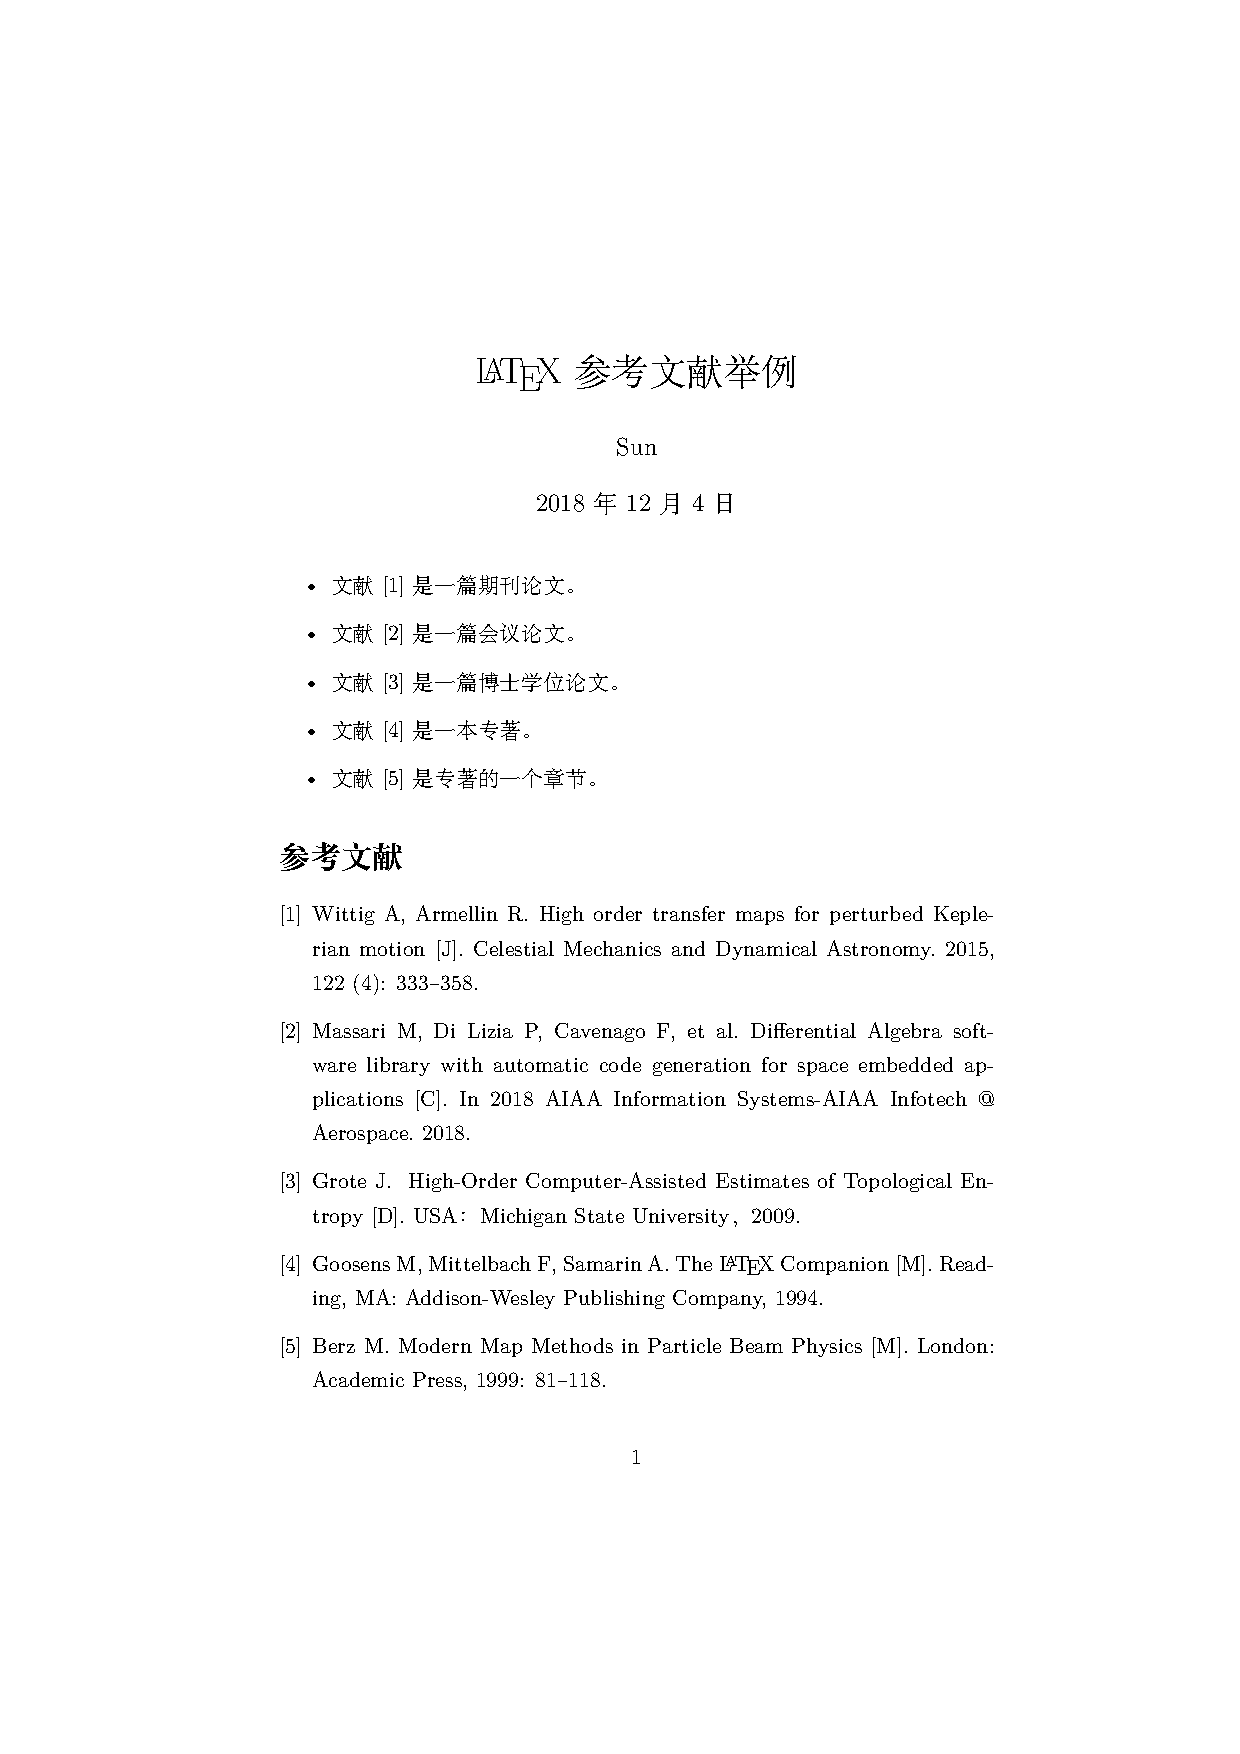
\includegraphics[width=0.9\textwidth]{example_ref/example_ref.pdf}
            \end{figure}
                }
            }
        \end{column}
    \end{columns}
\end{frame}

\begin{frame}{模板变更}
    \textcolor{red}{\emph{\LARGE{论文需要更换模板,怎样处理?}}}
    \begin{block}{Word}
        \begin{itemize}
            \item \textcolor{red}{按照模板,调整论文格式} \\
            逐项设置字体、段落、页面格式等,十分繁琐,容易遗漏
            \item \textcolor{red}{将论文内容复制到模板文件中} \\
            容易出现格式混乱、交叉引用错误等,需要重新排版
        \end{itemize}
    \end{block}
    \emph{\Large{在Word中,这是一项比较\textcolor{red}{耗时耗力}的工作}}
\end{frame}

\begin{frame}{模板变更}
    \textcolor{red}{\emph{\LARGE{论文需要更换模板,怎样处理?}}}
    \begin{block}{\LaTeX}
        \begin{itemize}
            \item 更换相应的模板
            \item 正文\textcolor{red}{不需修改或只要少量修改},快速完成格式转换
        \end{itemize}
    \end{block}
    \emph{\Large{在\LaTeX 中,这项工作可以\textcolor{red}{高效}地完成}} \\
\end{frame}

\begin{frame}[fragile]{模板变更}
    \begin{columns}
        \begin{column}{0.45\textwidth}
            会议论文模板
            \begin{lstlisting}
% 论文模板
\documentclass[paper,11pt]{IAA-AAS}
...
% 参考文献格式
\bibliographystyle{AAS_publication}
\PaperNumber{-x-xx} % 论文编号
...
% 作者信息
\author{San Zhang\thanks{Ph.D. ...}
}
...
            \end{lstlisting}
        \end{column}
        \begin{column}{0.45\textwidth}
            期刊论文模板
            \begin{lstlisting}
% 论文模板
\documentclass[3p,sort&compress]{elsarticle}
...
% 参考文献格式
\bibliographystyle{elsarticle-num}
\journal{Acta Astronautica} % 期刊名称
...
% 作者信息
\author[nudt_add]{San Zhang}
\ead{zhangsan@nudt.edu.cn}
\address[nudt_add]{College of ...}
...
            \end{lstlisting}
        \end{column}
    \end{columns}
\end{frame}

\begin{frame}{\LaTeX 核心思想}
    \begin{block}{内容与格式分离}
        \begin{itemize}
            \item \textcolor{red}{作者专注于文档的内容}
            \item 模板负责文档的格式
            \item \textcolor{red}{提高写作效率},不需为格式问题操心
            \item \textcolor{red}{所思即所得},有助于整理和构思文档的逻辑结构
        \end{itemize}
    \end{block}
\end{frame}


\section{怎样学习\LaTeX}

\begin{frame}{安装\LaTeX}
    \begin{block}{\LaTeX 发行版(必选)}
        \begin{itemize}
            \item 包含排版引擎(编译器)、文档类、模板、字体文件等
            \item TeX Live (Windows/Linux), MacTeX(Mac OS)
        \end{itemize}
    \end{block}
    \begin{block}{合适的文本编辑器(可选)}
        \begin{itemize}
            \item 有的编辑器提供一些增强功能,使用更加方便
            \item TeXstudio, VS Code, Vim, ...
        \end{itemize}
    \end{block}
\end{frame}

\begin{frame}{\LaTeX 学习方法}
    \begin{block}{网上找一个简单的例子,自己实现一遍}
        \begin{itemize}
            \item 了解LaTeX文档的结构,基本的语法,生成pdf的过程
        \end{itemize}
    \end{block}
    \begin{block}{浏览几篇比较好的参考资料,了解\LaTeX 主要功能}
        \begin{itemize}
            \item 官方文档、lnotes2、lshort-zh-cn
        \end{itemize}
    \end{block}
    \begin{block}{\textcolor{yellow}{边用边学},是最好的学习方式}
        \begin{itemize}
            \item 从下一篇小论文开始,考虑使用LaTeX编写
            \item 找一份现成的源文件作为参考,替换为自己的论文内容
            \item 遇到问题,再去翻阅参考资料
        \end{itemize}
    \end{block}
\end{frame}


\section{总结}

\begin{frame}{\secname}
    \begin{block}{\textcolor{yellow}{磨刀不误砍柴工}}
        \begin{itemize}
            \item 相比已经很熟练的Word,刚开始用LaTeX时效率低
            \item 坚持不断使用,越来越熟练,效率越来越高
            \item 写论文时不再需要操心格式问题,获得更高的工作效率
        \end{itemize}
    \end{block}
    \begin{block}{拓展功能}
        \begin{itemize}
            \item 制作\textcolor{red}{幻灯片、信函、简历}等
            \item \textcolor{red}{本文档}由\LaTeX 生成
        \end{itemize}
    \end{block}
\end{frame}


\section{Q\&A}
\begin{frame}{\secname~ }
	\begin{center}
 		\huge {\kaishu 结束,谢谢}
		
		\huge \textit {Q\&A}
	\end{center}
\end{frame}
\end{document}
